This section describes the dataset, evaluation metrics, and experimental procedure used in this study.

\subsection{Dataset}

In this study, we used three types of Python project configurations as the dataset:

\begin{enumerate}
    \item Prompt + Docstrings \footnote{\url{https://github.com/soso0024/pj-aidev-dataset_prompt_docstrings}}
\vspace{0.2cm}
    \item Prompt Only \footnote{\url{https://github.com/soso0024/pj-aidev-dataset_prompt_only}}
\vspace{0.2cm}
    \item Compressed Prompt + Comprssed Docstrings (by LLMLingua-2) \footnote{\url{https://github.com/soso0024/pj-aidev-dataset_llmlingua-2}}
\end{enumerate}

Each configuration maintains identical function and class structures as well as dependency relationships. Only one factor changes are that whether the prompt and its Docstrings are included and compressed. This setup allows for controlled evaluation of how natural language documentation—and its compression—affects the performance of LLM-based test case generation. 

The dataset emulates a complete financial-transaction workflow—user signup/login, balance tracking, payment processing, and order history—all on in-memory storage. The dataset offers the following key features:

\begin{itemize}[label={$\bullet$}]
    \item \textbf{Project Structure}:\\Each project is composed of the following directories: config/, data/, model/, repository/, service/, and utils/. Fig.\ref{fig:repository_visualization} shows a project visualization of the repository used in this study.
\vspace{0.2cm}
    \item \textbf{Code Formatting}:\\All repositories were formatted using Black to ensure consistent code style \footnote{\url{https://github.com/psf/black}}. Deviations from the formatting standard are detected via GitHub Actions using black\_formatter.yml. This enforcement ensures that differences in code style do not influence the experimental results.
\end{itemize}

\begin{figure}[htbp]
    \centering
    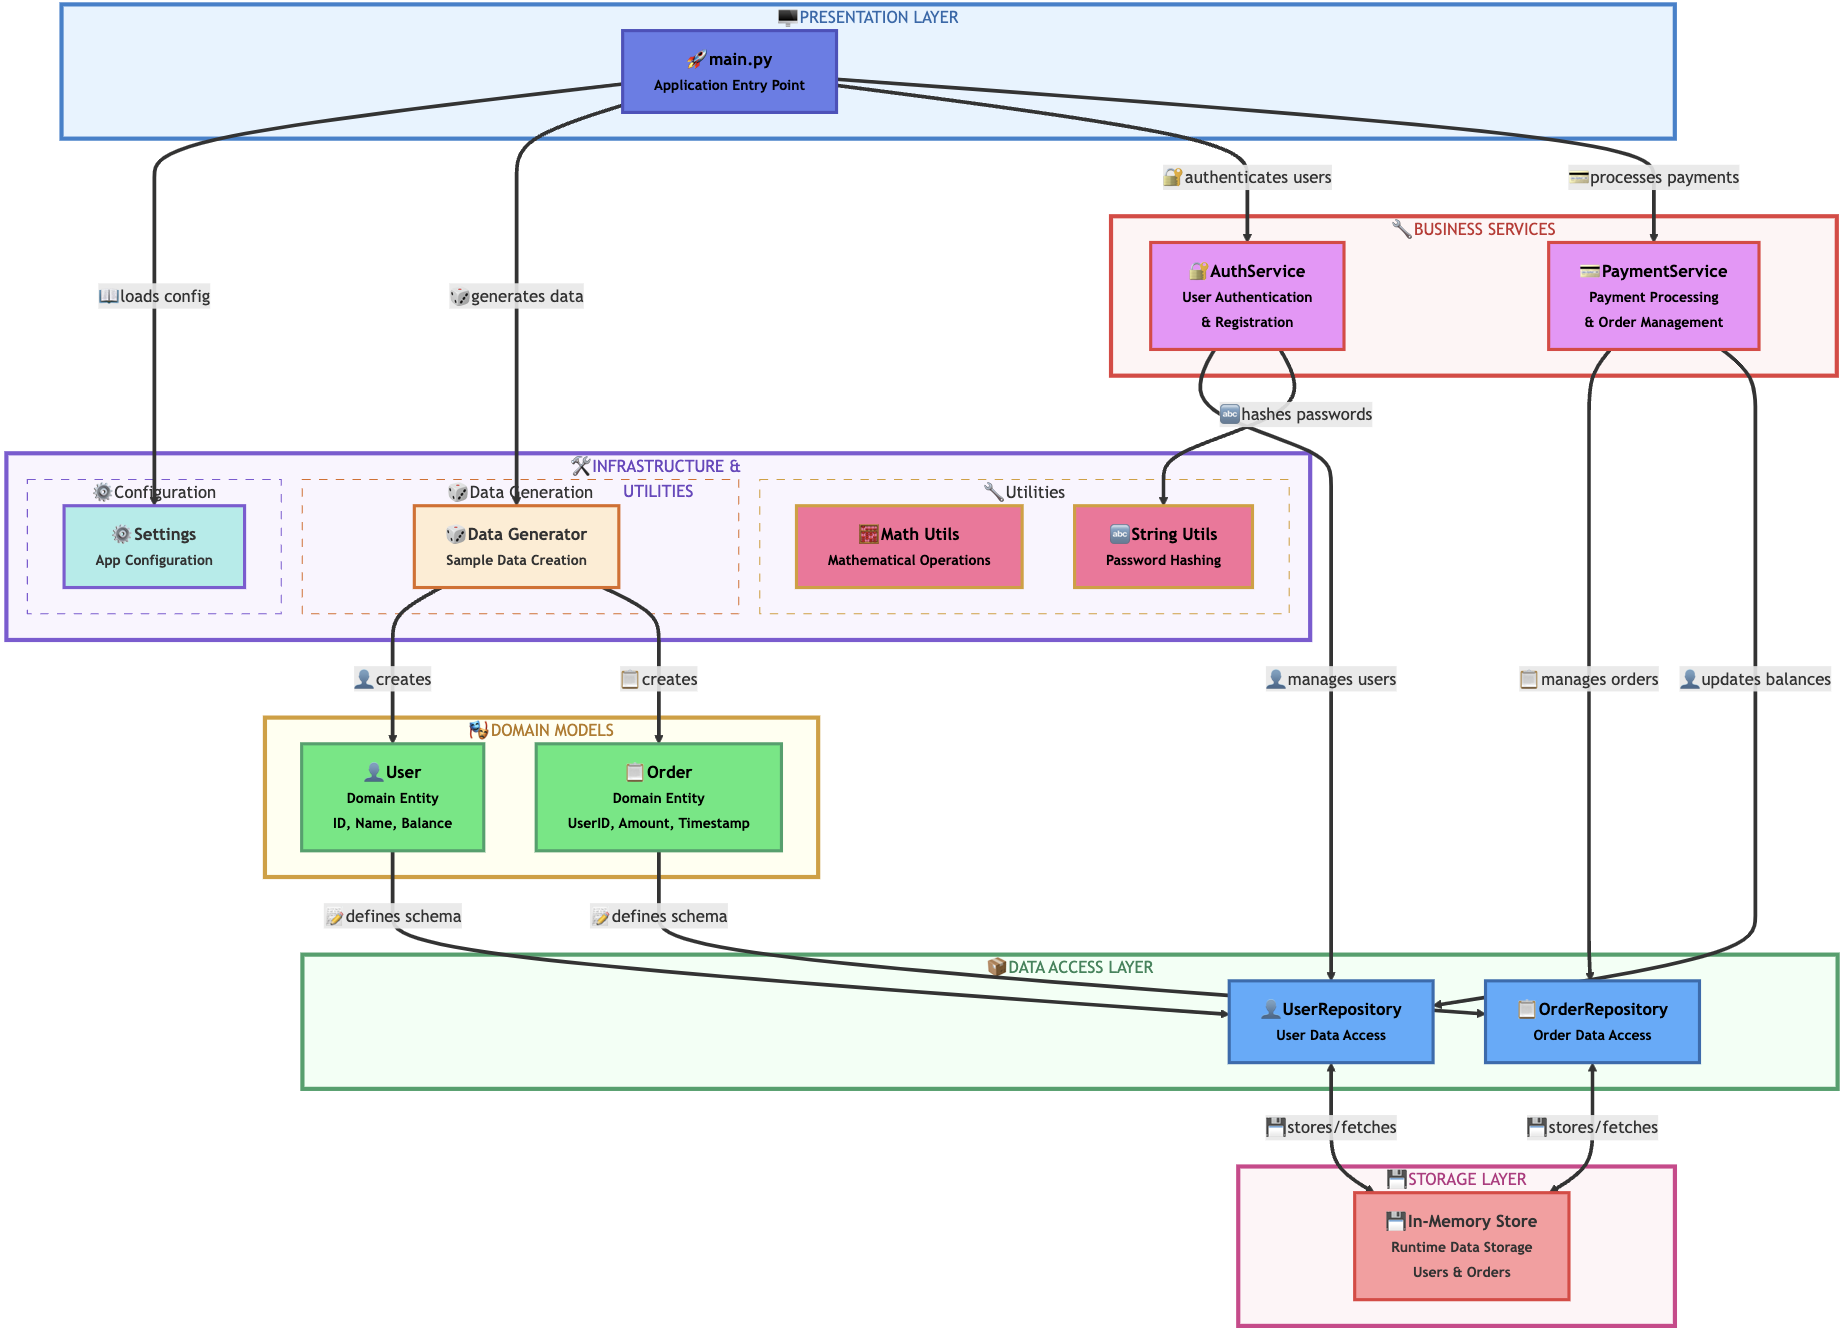
\includegraphics[width=1.09\linewidth]{imgs/eps/repository_visualization.eps}
    \caption{Project Repository Visualization}
    \label{fig:repository_visualization}
\end{figure}

Through these measures, we constructed a dataset that enables systematic evaluation of the impact of natural language and compression of natural language on test generation.

\subsection{Evaluation Metrics}

In this experiment, we evaluated performance using the following three primary metrics: token count, API cost, and code coverage.

\begin{enumerate}
    \item Token Counts + API Costs
\vspace{0.2cm}
    \item Number of Requests
\vspace{0.2cm}
    \item Code Coverage
\end{enumerate}

During the experiment, we recorded the cumulative token count and API cost required for Cline to generate and iteratively refine test code until it executed without errors. These values were compared against the final achieved values for each configuration.

The total token count per input prompt is defined as:

\[
\text{Input Prompt}
  = \text{Source Code}
  + \text{Prompt}
  + \text{Docstrings (if present)}
  + \text{Error Report}
\]

\subsection{Experimental Procedure}
Figure \ref{fig:experiment_overview} shows the overall experimental procedure. As shown by the structure of the dataset, we evaluated three different test case generation methods using LLMs:

\begin{figure}[htbp]
    \centering
    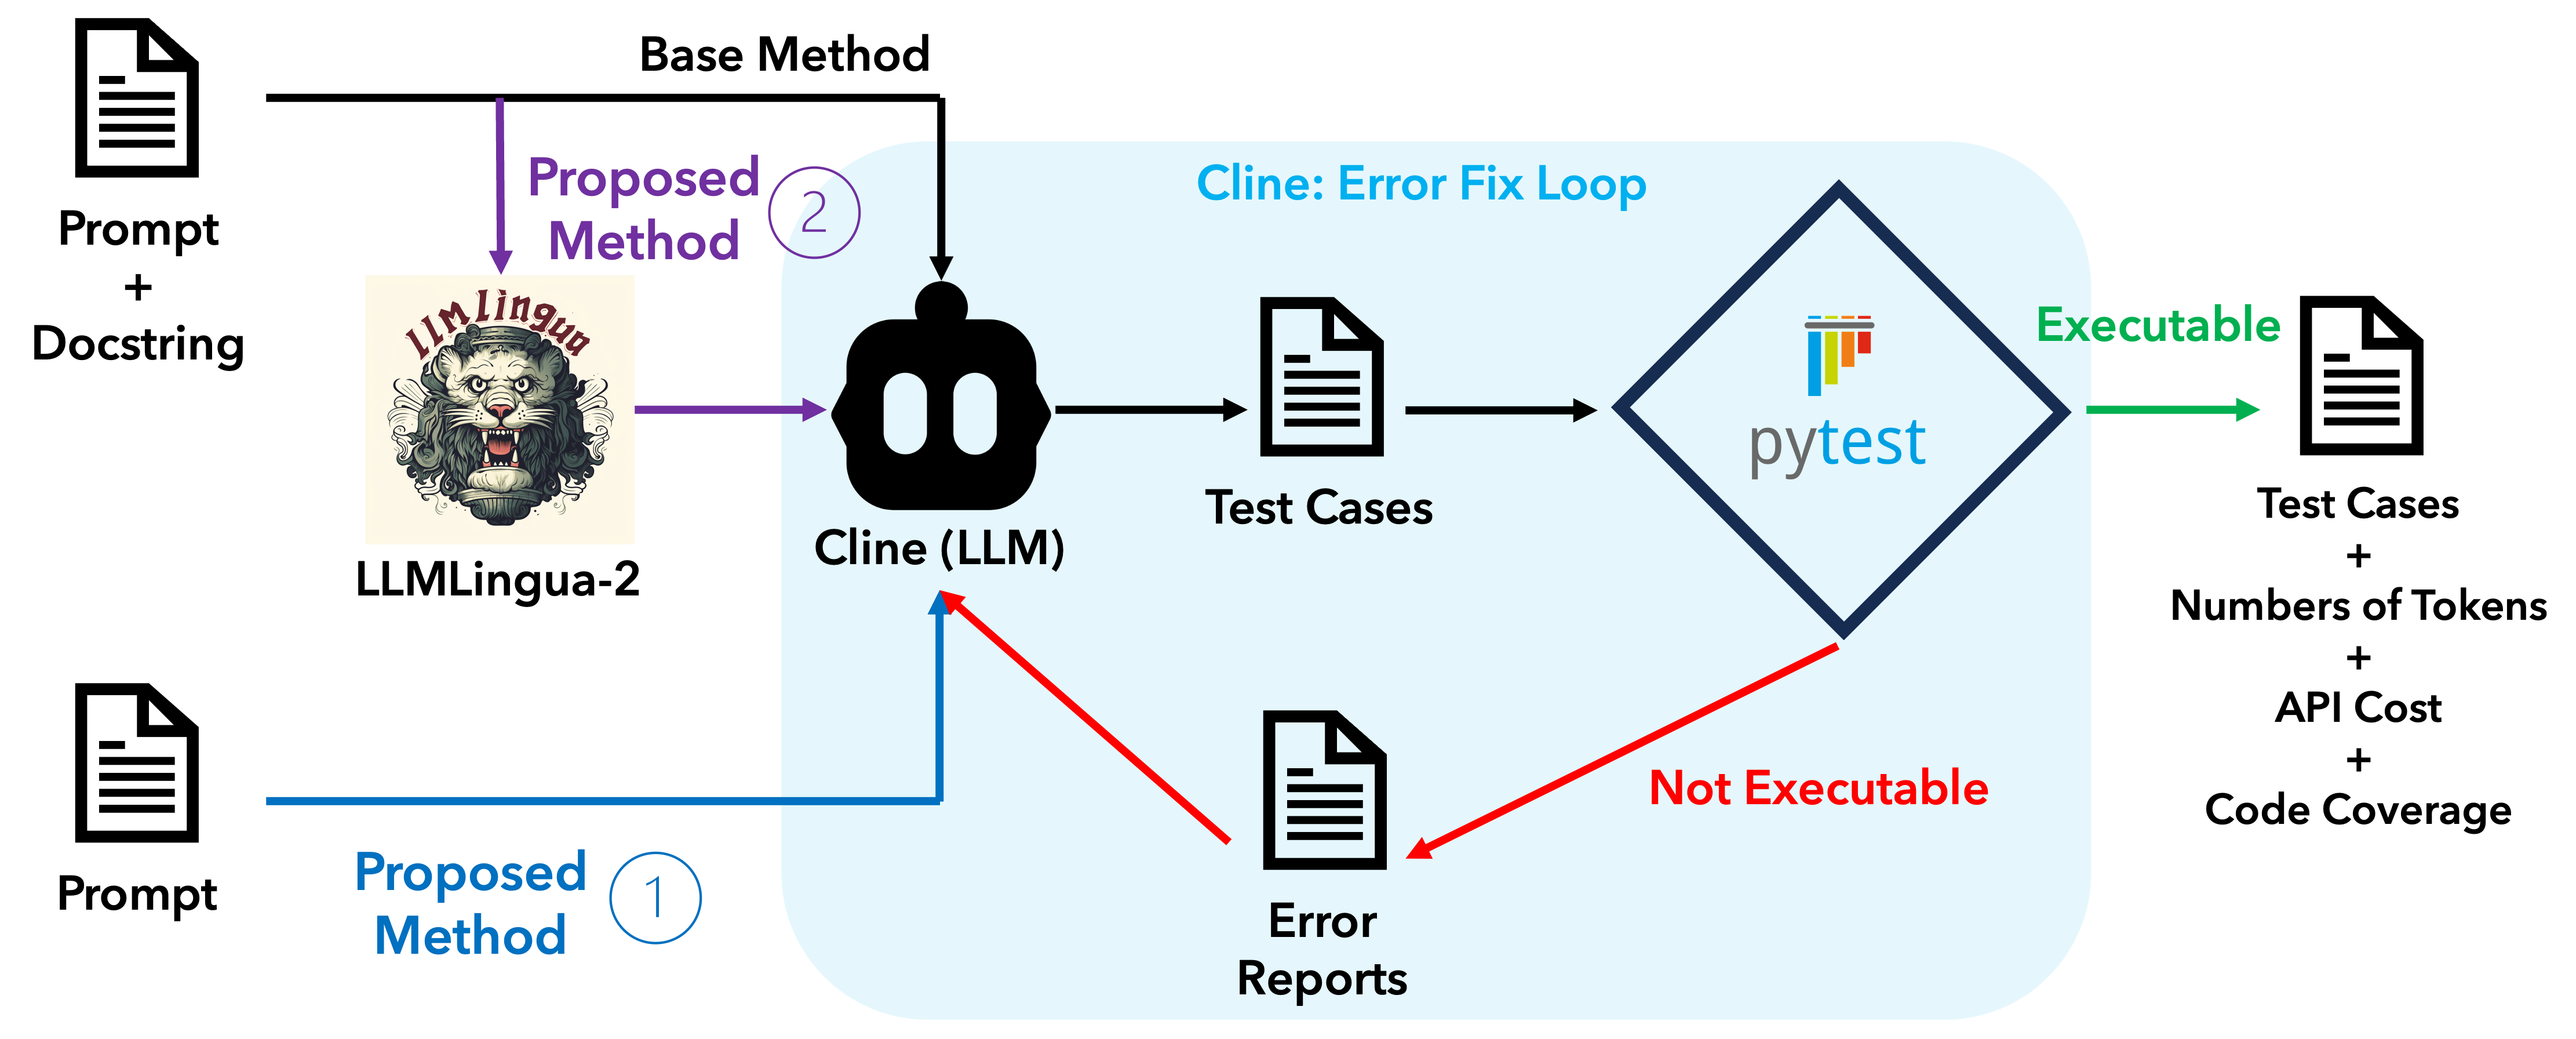
\includegraphics[width=1.0\linewidth]{imgs/png/overview_old.png}
    \caption{Experiment Overview}
    \label{fig:experiment_overview}
\end{figure}

\begin{itemize}[label={$\bullet$}]
    \item \textbf{Base Method}: \\Test cases are generated by providing LLMs with source code that includes both the prompt and Docstrings.
\vspace{0.2cm}
    \item \textbf{Proposed Method 1}: \\Docstrings are removed from the code, and only the prompt is provided to LLMs.
\vspace{0.2cm}
    \item \textbf{Proposed Method 2}: \\The same prompt and Docstrings used in the Base Method are compressed using LLMLingua-2 before being provided to LLMs.
\end{itemize}

As described earlier, an AI agent framework is used to iteratively generate and fix test cases until they execute correctly. The correctness of generated test cases is verified using a Pytest-based environment.
